\chapter{Progettazione dell'algoritmo}
\label{cap:analisi-requisiti}

\lstset{
    escapeinside={(*@}{@*)}, % Delimitatori per modalità LaTeX
    basicstyle=\ttfamily,    % Stile monospaziato
}

\intro{Questo capitolo è incentrato sulla progettazione e sulla calibrazione dei parametri dell'algoritmo}

\section{Progettazione}

Questa sezione esplora i diversi aspetti fondamentali nella progettazione di un algoritmo genetico: le componenti fondamentali, la struttura e gli operatori genetici.

\subsection{Composizione degli algoritmi evolutivi} \hypertarget{elementi}{}

I principali componenti di ricerca per progettare un algoritmo evolutivo sono i seguenti [\hyperlink{bibliografia}{1}]:

\begin{itemize}
    \item \textbf{Rappresentazione}: negli algoritmi genetici, la soluzione codificata è chiamata cromosoma, mentre le variabili decisionali all'interno di una soluzione (cromosoma) sono i geni;
    
    \item \textbf{Inizializzazione della popolazione}: la generazione della popolazione iniziale è un aspetto cruciale in quanto una giusta inizializzazione determina un vantaggio già dalle prime iterazioni;
    
    \item \textbf{Funzione di fitness}: si tratta della funzione obiettivo, ogni soluzione ha un valore di fitness che indica il grado di adeguatezza rispetto al problema;
    
    \item \textbf{Strategia di selezione}: la strategia di selezione affronta la seguente domanda: "Quali genitori per la prossima generazione vengono scelti con un bias verso un fitness migliore?";
    
    \item \textbf{Strategia di riproduzione}: la strategia di riproduzione consiste nel progettare operatori di mutazione e crossover adeguati per generare nuovi individui (discendenti);
    
    \item \textbf{Strategia di sostituzione}: i nuovi discendenti competono con gli individui più vecchi per ottenere il loro posto nella prossima generazione (sopravvivenza del più adatto);
    
    \item \textbf{Criteri di arresto}: determina la fine del loop evolutivo, solitamente è indicato come il numero di generazioni da raggiungere, ovvero ogni iterazione è una generazione.
\end{itemize}

\subsection{Base dell'algoritmo genetico} \hypertarget{ga}{}

In questa sezione descriviamo la struttura dell'Algoritmo Genetico scelta per il controllo delle sue fasi di intensificazione e diversificazione [\hyperlink{bibliografia}{4}].
L'obiettivo è massimizzare una funzione di fitness $f$. I parametri richiesti dall'algoritmo GA sono:

\begin{itemize}
    \item $N$: dimensione della popolazione;
    \item $p_c$: probabilità di crossover;
    \item $p_m$: probabilità di mutazione;
    \item $M$: dimensione del pool di accoppiamento;
    \item $E$: dimensione dell'élite.
\end{itemize}

Indichiamo con $P$ la popolazione di cromosomi e con $G$ l'insieme di discendenti generati dalla fase di riproduzione. Di segito è presente il pseudocodice della funzione GA, per favorire una lettura immediata della struttura dell'algoritmo, evidenziando i passaggi più importanti, ovvero: generazione della popolazione iniziale, riproduzione e rimpiazzo.

\begin{lstlisting}
def GA(N, pc, pm, M, E):
    P = generate(N);
    while not terminate() do
        G = reproduction(P, pc, pm, M);
        P = replace(P, G, E);
    end
    return maxf P;
end
\end{lstlisting}

\subsubsection{Riproduzione}
In questa fase utilizziamo operatori binari (crossover) e unari (mutazione) per esplorare altre soluzioni alterando solo una parte della soluzione. Questa modifica parziale (invece di una riorganizzazione totale, che sarebbe una ricerca casuale), insieme al sostegno degli individui più idonei (es. selezione dei genitori), porta l'algoritmo a spingere avanti nelle generazioni le soluzioni più idonee mantenendo un buon tasso di esplorazione di nuovi cromosomi. La dimensione dei discendenti richiesta è pari alla dimensione della popolazione $N$, che poi subisce la procedura di sostituzione.

La probabilità di riproduzione indicata con $Be(p)$, ovvero, la variabile casuale di Bernoulli che assume valore 1 con probabilità $p$ e 0 con probabilità $1-p$. Di segito è presente lo pseudocodice della funzione Reproduction.

\begin{lstlisting}
    def Reproduction(P, pc, pm, M):
        G = [ ];
        pool = sortf(P)[0 : M];
        while not |G| == |P| do
            par1, par2 = selection(pool);
            if Be(pc) == 1 then
                c1, c2 = crossover(par1, par2);
            else
                c1, c2 = par1, par2;
            end
            G = G (*@$\cup$@*) {c1, c2};
        end
        foreach g (*@$\in$@*) G do
            if Be(pm) == 1 then
                mutation(c);
            end
        end
        return G;
    end
\end{lstlisting}

\subsubsection{Rimpiazzo}
La strategia di rimpiazzo ha un grande impatto sull'intensificazione. La metodologia di rimpiazzo adottata può essere spiegata in due passaggi: 
\begin{enumerate}
    \item i migliori $E$ elementi nell'unione di $P$ e $G$ fanno automaticamente parte della popolazione successiva;
    \item i migliori $|P| - E$ discendenti di $G$ sono inclusi nella popolazione successiva.
\end{enumerate}

\noindent Di segito è presente lo pseudocodice della funzione Replace.

\begin{lstlisting}
    def Replace(P, G, E):
        elite = best subset(P (*@$\cup$@*) G, E, f);
        Gbest = best subset(G, |P| - E, f);
        return elite (*@$\cup$@*) Gbest;
    end
\end{lstlisting}

\subsection{Operatori genetici} \hypertarget{og}{}

Gli operatori genetici permettono agli algoritmi evolutivi di modulare la diversificazione. Operano sui cromosomi alterandone i geni e permettendo di esplorare un ampio spazio di soluzioni senza andare a perdere intensificazione grazie alla selezione e all'elitismo. Le informazioni e immagini riportate in questa sezione sono prese da Metaheuristics di El-Ghazali Talbi [\hyperlink{bibliografia}{1}].

\subsubsection{Selezione}

La selezione dei genitori viene effettuata sui migliori \( M \) individui della popolazione attuale, i quali costituiscono il cosiddetto \emph{Mating Pool}.

Il meccanismo di selezione è uno dei principali componenti di ricerca negli algoritmi evolutivi (EAs). Il principio fondamentale dei metodi di selezione è: \emph{"più un individuo è valido, maggiore è la sua probabilità di essere scelto come genitore."} Questa pressione selettiva guida la popolazione verso soluzioni migliori. Tuttavia, gli individui peggiori non dovrebbero essere completamente scartati, poiché essi potrebbero contenere materiale genetico utile.

La strategia di selezione determina quali individui vengono scelti per l'accoppiamento (riproduzione).

La selezione tramite ruota della roulette è la strategia di selezione più comune. Essa assegna a ciascun individuo una probabilità di selezione proporzionale alla sua fitness relativa (Figura 4.1). Sia $f_i$ la fitness dell'individuo $p_i$ nella popolazione $P$. La probabilità di selezione è data da:

\[ p_i = \frac{f_i}{\sum_{j=1}^{n} f_j} \]

Immaginiamo un grafico a torta in cui a ciascun individuo è assegnato uno spazio proporzionale alla sua fitness. Una ruota della roulette è posizionata attorno al grafico. La selezione di $\mu$ individui avviene tramite $\mu$ spin indipendenti della ruota. Ogni spin seleziona un singolo individuo. Gli individui migliori occupano più spazio e, di conseguenza, hanno maggiori probabilità di essere scelti (Figura 4.2).
\hypertarget{img6}{}
\begin{figure}[!ht] 
    \centering 
    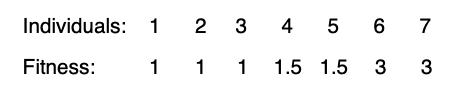
\includegraphics[width=0.6\columnwidth]{tesi/fitness_roulette_wheel} 
    \caption[Pesi della ruota]{Pesi della ruota [\hyperlink{bibliografia}{1}]}
\end{figure}

\hypertarget{img7}{}
\begin{figure}[!ht] 
    \centering 
    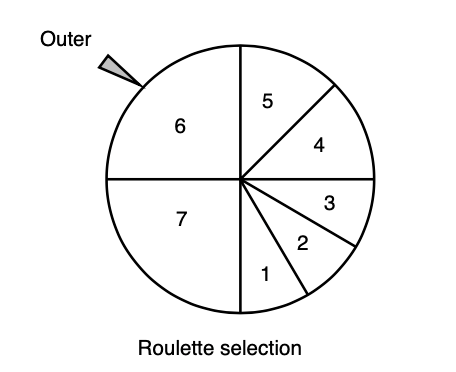
\includegraphics[width=0.6\columnwidth]{tesi/roulette_wheel} 
    \caption[Grafico a torta della selezione tramite ruota della roulette]{Grafico a torta della selezione tramite ruota della roulette [\hyperlink{bibliografia}{1}]}
\end{figure}

Tuttavia, nella selezione tramite ruota della roulette, individui eccezionali possono introdurre un bias all'inizio della ricerca, causando una convergenza prematura e una perdita di diversità genetica. Infatti, va notato che un valore di \( M \) troppo piccolo intensifica il focus sui migliori individui del \emph{Mating Pool}, riducendo però la diversificazione della popolazione. Questo compromesso deve essere attentamente bilanciato per garantire un efficace equilibrio tra esplorazione e sfruttamento nel processo evolutivo.

\subsubsection{Crossover}
Il crossover prende i due genitori selezionati e genera due figli da aggiungere ai nuovi discendenti. Un crossover avviene con una probabilità $p_c$, altrimenti i genitori vengono semplicemente clonati e aggiunti ai discendenti. L'operatore di crossover, da un lato, mescola i geni delle coppie di cromosomi esplorando nuove soluzioni; dall'altro, se la diversità genetica (individui diversi) nella popolazione è bassa, può portare a una convergenza prematura. Nel caso estremo in cui abbiamo una popolazione composta da elementi tutti uguali, il crossover non può creare nuovi individui. Per garantire la diversità genetica, si può ridurre la fase di intensificazione (es. $E$ o $M$) o aumentare il tasso di mutazione $p_m$.

A differenza degli operatori unari, come la mutazione, l'operatore di crossover è binario e talvolta n-ario. Il ruolo degli operatori di crossover è di ereditare alcune caratteristiche dei due genitori per generare i discendenti. Come per l'operatore di mutazione, la progettazione degli operatori di crossover dipende principalmente dalla rappresentazione utilizzata.

Applicare operatori di crossover classici alle permutazioni, come nel nostro caso, genera soluzioni che non sono permutazioni (ossia, soluzioni non valide). Di conseguenza, sono stati progettati numerosi operatori di crossover per permutazioni, tra cui il crossover a ordine (OX - order crossover) (Figura 4.3). Per prima cosa, due punti di crossover vengono selezionati casualmente. Dal genitore 1, si copia nel discendente, alle stesse posizioni assolute, la parte tra i due punti. Dal genitore 2, si parte dal secondo punto di crossover e si scelgono gli elementi non già selezionati dal genitore 1, inserendoli nel discendente a partire dal secondo punto di crossover. L'operatore di crossover OX è un operatore di pura ricombinazione. Se si inizia a riempire o scegliere dal primo punto di crossover, l'operatore non sarà puro. Dal genitore 1, vengono preservati l'ordine relativo, l'adiacenza e le posizioni assolute. Dal genitore 2, viene preservato solo l'ordine relativo. 

\begin{figure}[!ht] 
    \centering 
    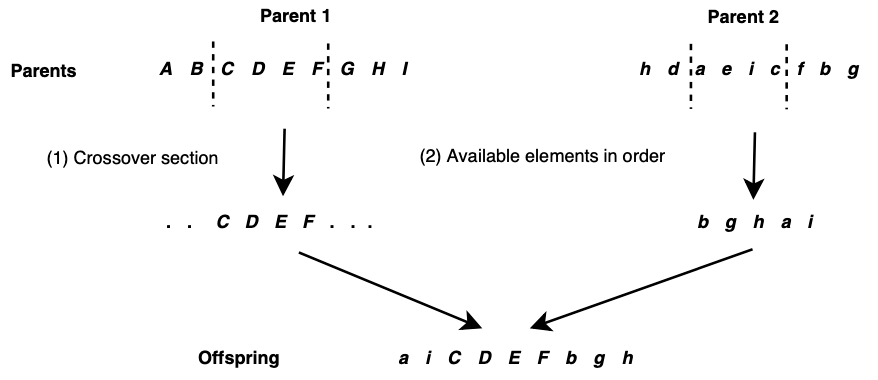
\includegraphics[width=1\columnwidth]{tesi/OXCrossover} 
    \caption[Rappresentazione del crossover OX]{Rappresentazione del crossover OX [\hyperlink{bibliografia}{2}]}
\end{figure}

\subsubsection{Mutazione}
La mutazione viene eseguita dopo il crossover e crea una perturbazione casuale del cromosoma selezionato. Il ruolo della mutazione è duplice: da un lato, simile all'operatore di crossover, provoca una perturbazione di una soluzione per favorire l'esplorazione; dall'altro aumenta la diversità genetica anche se l'attuale diversità è scarsa. Questo è in contrasto con il crossover, che non può diversificare molto un set di individui molto simili.

Gli operatori di mutazione sono operatori unari che agiscono su un singolo individuo. Le mutazioni rappresentano piccoli cambiamenti degli individui selezionati nella popolazione. La probabilità $p_m$ definisce la probabilità di mutare ogni elemento (gene) della rappresentazione. Alcune strategie inizializzano la probabilità di mutazione a $1/k$, dove $k$ è il numero di variabili decisionali, in modo che in media solo poche variabili vengano mutate.

Alcuni punti importanti da considerare nella progettazione o nell'uso di un operatore di mutazione sono i seguenti:

\begin{itemize}
    \item \textbf{Ergodicità}: l'operatore di mutazione dovrebbe consentire di raggiungere ogni soluzione nello spazio di ricerca.
    \item \textbf{Validità}: l'operatore di mutazione dovrebbe produrre soluzioni valide. Questo non è sempre possibile nei problemi di ottimizzazione vincolati.
    \item \textbf{Località}: la mutazione dovrebbe produrre un cambiamento minimo. La dimensione della mutazione è importante e dovrebbe essere controllabile. La località è l'effetto sulla soluzione (fenotipo) quando si esegue la modifica (perturbazione) nella rappresentazione (genotipo). Quando vengono effettuati piccoli cambiamenti nel genotipo, il fenotipo deve rivelare piccoli cambiamenti. In questo caso, si dice che la mutazione ha una forte località. Una debole località è caratterizzata da un grande effetto sul fenotipo quando viene effettuato un piccolo cambiamento nel genotipo.
\end{itemize}

La mutazione in rappresentazioni basate sull'ordine, come nel nostro caso, è generalmente basata sugli operatori di scambio (swapping), inversione o inserimento. 

\section{Calibrazione dei parametri}

In questa sezione viene discussa e motivata la scelta dei valori dei parametri dell'algoritmo tenendo contro delle caratteristiche da ottimizzare, delle istanze di prova fornite dall'azienda e di possibili rischi di overfitting.

L'obiettivo è quello scegliere una configurazione ottimale di parametri dell'algoritmo per cercare di bilanciare le seguenti caratteristiche:
\begin{itemize}
	\item\textbf{Intensificazione}: ci si aspetta che il valore di fitness della soluzione migliore all'interno della popolazione incrementi nel corso delle generazioni;
	\item\textbf{Diversificazione}: l'algoritmo deve esplorare un vasto insieme di soluzioni, gli operatori di crossover e mutazione potranno generare soluzioni con valori fitness inferiori a quello della peggiore soluzione della generazione precedente. Quando questo avviene significa che l'algoritmo sta esplorando anche soluzioni diverse, tuttavia non è necessariamente indice che l'esplorazione avvenga in maniera sufficente;
	\item\textbf{Costo computazionale}: come vedremo in seguito, il criterio di arresto dei test svolti sull'algoritmo è un limite di tempo impostato a 30 secondi, imposto dal contesto di utilizzo. In base all'istanza, è possibile che in 30 secondi vengano calcolate 10 o 100 generazioni. La qualità della soluzione ottenuta solitamente dipende dal numero di generationi. Questo rende la velocità di esecuzione un aspetto di cui tenere conto per permettere all'algoritmo di eseguire più generazioni possibili nel tempo limite.
\end{itemize}

\subsection{Scelta delle configurazioni}

I parametri da configurare sono:
\begin{itemize}
	\item\textbf{population\_size}: dimensione della popolazione di cromosomi, ovvero le soluzioni sul quale lavora il genetico;
	\item\textbf{crossover\_prob}: probabilità che l'algoritmo svolga l'operazione di crossover (applicata a coppie di soluzioni presenti nella pool);
	\item\textbf{mutation\_prob}: probabilità che l'algoritmo svolga l'operazione di mutazione (applicata a ogni soluzione presente nella pool);
	\item\textbf{mating\_pool\_size}: dimensione del pool di accoppiamento;
	\item\textbf{elite\_size}: dimensione dell'insieme dei migliori cromosomi della popolazione che verranno inseriti direttamente nella popolazione della generazione successiva.
\end{itemize}

\noindent La configurazione iniziale (fornita dal tutor aziendale sulla base risultati ottenuti per un algoritmo genetico svolto su un altro problema) è, \textbf{Conf1}:
\begin{itemize}
	\item\textbf{population\_size}: 50;
	\item\textbf{crossover\_prob}: 0,7 (70\%);
	\item\textbf{mutation\_prob}: 0,3 (30\%);
	\item\textbf{mating\_pool\_size}: 20;
	\item\textbf{elite\_size}: 5.
\end{itemize}

Di seguito verranno mostrati alcuni grafici di test svolti su delle singole istanze di prova, fornite appositamente dall'azienda, allo scopo di mostrare l'andamento del valore di fitness delle soluzioni della determinata istanza. Inoltre, per i test sui parametri dell'algoritmo è stato imposto un criterio di arresto non a limite di tempo ma a limite di generazioni, ed è stato fissato a 50 generazioni. 
L'asse y rappresenta il valore di fitness (da 0.75 a 0.95, dove 0 significa che lo spazio sprecato è tutto, e 1 che non c'è spazio sprecato). L'asse x rappresenta il numero di generazioni (da 0 a 50).
La trasparenza è regolata in modo che più sono presenti cromosomi maggiore è l'intensità del blu.

Dal seguente grafico (Figura 4.4) si nota come ci sia una buona diversificazione ma il valore di fitness della soluzione migliore converge troppo presto, infatti, intorno alla 15esima generazione stabilizza il valore di fitness della soluzione migliore. 

\begin{figure}[!ht] 
    \centering 
    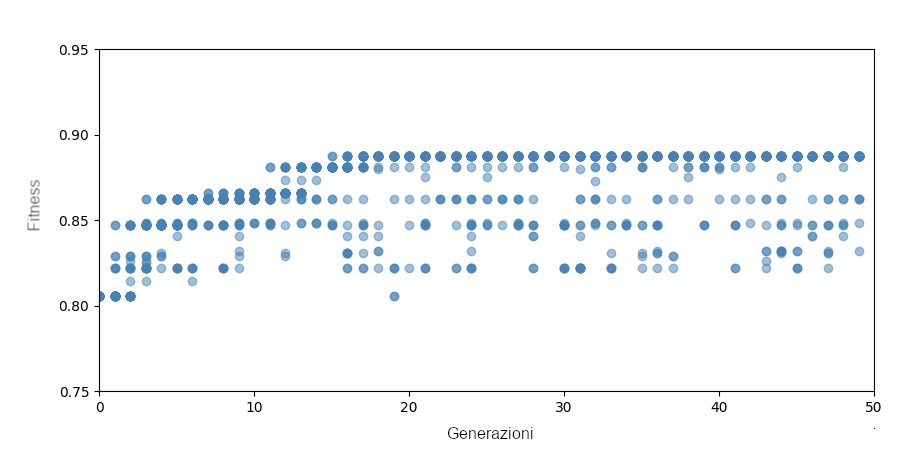
\includegraphics[width=1\columnwidth]{tesi/conf1} 
    \caption{Andamento valori di fitness di un instanza di prova testata con Conf1}
\end{figure}

Ulteriori test sono stati eseguiti con la \textbf{Conf2}:
\begin{itemize}
	\item\textbf{population\_size}: 50;
	\item\textbf{crossover\_prob}: 0,7 (70\%);
	\item\textbf{mutation\_prob}: 0,3 (30\%);
	\item\textbf{mating\_pool\_size}: 40;
	\item\textbf{elite\_size}: 5.
\end{itemize}

Per cercare subito un confronto la prima modifica è stata nella \emph{mating\_pool\_size}, portandola a 40 (da 20) (Figura 4.5), questo ha aumentato notevolmente la diversificazione ed ha trovato soluzioni con un valore di fitness migliore delle soluzioni migliori con la Conf1. 

\begin{figure}[!ht] 
    \centering 
    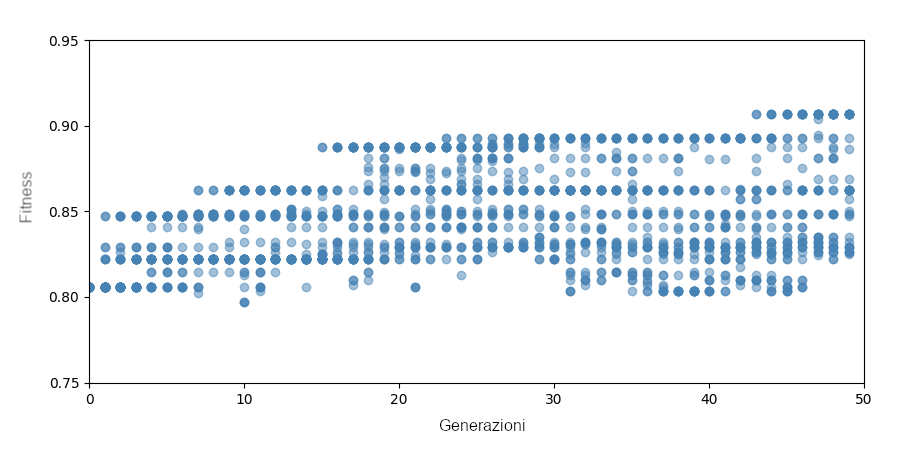
\includegraphics[width=1\columnwidth]{tesi/conf2} 
    \caption{Andamento valori di fitness di un instanza di prova testata con Conf2}
\end{figure}

Questo ha indicato come sicuramente sono presenti soluzioni migliori ottenibili con lo stesso numero di generazioni. Come si può notare, la Conf2 ha molta diversificazione, quindi l'obiettivo di una nuova configurazione era migliorare l'intensificazione e cercare di diminuire la diversificazione senza perdere le nuove soluzioni che hanno ottenuto un valore di fitness migliore. Si è provato a diminuire la \emph{mating\_pool\_size} e aumentare la \emph{elite\_size} per aumentare l'intensificazione, ma è stato chiaro da subito che un 10\% di \emph{elite\_size} era già il massimo ottenibile senza ridurre drasticamente la diversificazione. Quindi si è provato ad aumentare \emph{crossover\_prob} ma con scarso successo. Sono state tentate anche configurazioni con diverse \emph{mutation\_prob} ma diminuendola si notava chiaramente un appiettimento della diversificazione, mentre, non si rendeva necessario aumentarla dato che un aumento della \emph{mating\_pool\_size} è sufficente per ottenere un giusto livello di diversificazione e aumenta anche l'intensificazione grazie al crossover.

\noindent L'equilibrio è stato trovato con la \textbf{Conf3}:
\begin{itemize}
	\item\textbf{population\_size}: 50;
	\item\textbf{crossover\_prob}: 0,7 (70\%);
	\item\textbf{mutation\_prob}: 0,3 (30\%);
	\item\textbf{mating\_pool\_size}: 30;
	\item\textbf{elite\_size}: 5.
\end{itemize}

La Figura 4.6 mostra l'andamento dei valori di fitness di un test con la configurazione 3, che ha una \emph{mating\_pool\_size} corrispondente al 60\% della popolazione, che genera un bilanciamento ottimale fra intensificazione, diversificazione e velocità di esecuzione. Infatti, un altro problema della Conf2 era che una \emph{mating\_pool\_size} di 40 faceva svolgere una generazione in molto più tempo rispetto alla Conf1, quindi, siccome i test di confronto con la soluzione aziendale sarebbero stati svolti non con un criterio di arresto basato sulle generazione ma sul tempo, è stato necessario diminuire la \emph{mating\_pool\_size}.

\begin{figure}[!ht] 
    \centering 
    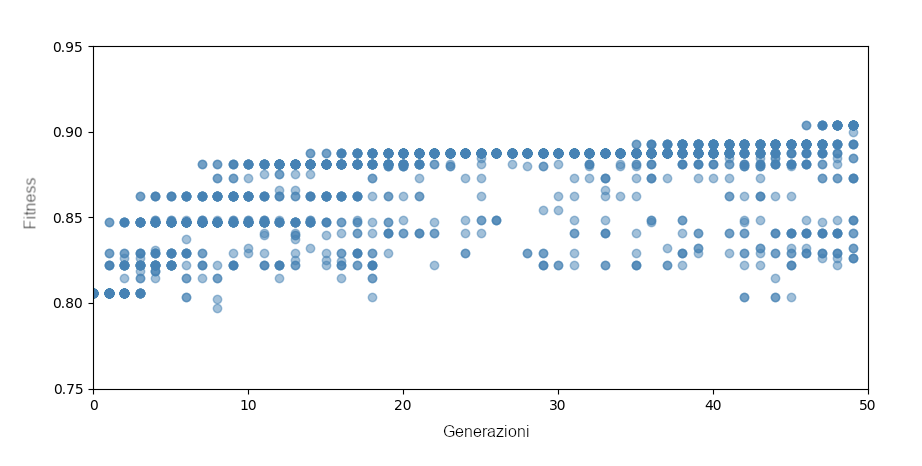
\includegraphics[width=1\columnwidth]{tesi/conf3} 
    \caption{Andamento valori di fitness di un instanza di prova testata con Conf3}
\end{figure}

\subsection{Confrontro tra configurazioni di parametri} \hypertarget{ttest}{}

Per confrontare le configurazioni, sono state generate randomicamente 50 istanze di prova diverse, ciascusa istanza ha:
\begin{itemize}
	\item 1 solo tipo di foglio;
	\item 20 item obbligatori più 0 o 6 o 12 item opzionali;
	\item 0 o metà o tutti gli item obbligatori di una classe hanno margini;
	\item 0 o 20 precedenze, ovvero o nessun item obbligatorio ha precedenze oppure tutti gli obbligatori hanno una precedenza diversa.
\end{itemize}

Le seguenti medie sono ottenute sui valori di fitness della soluzione miglire, per ogni istanza, e il tempo (in secondi) impiegato per eseguire le 50 generazioni.

\begin{itemize}
    \item \textbf{Conf1}
    \begin{itemize}
        \item\textbf{Fitness}: 0.7785907496795459
        \item\textbf{Tempo}: 26.64 
    \end{itemize}
    \item \textbf{Conf2}
    \begin{itemize}
        \item\textbf{Fitness}: 0.7804101596824722
        \item\textbf{Tempo}: 27.76
    \end{itemize}
    \item \textbf{Conf3}
    \begin{itemize}
        \item\textbf{Fitness}: 0.780764190701669
        \item\textbf{Tempo}: 27.26
    \end{itemize}
\end{itemize}

Si può notare che da questi risultati che la configurazione migliore risulta essere la 3, tuttavia di tratta solo di risultati basati su determinate istanze. È importante sottolineare che tramite un \emph{t-test}\glsfirstoccur non sono stati rilevati sufficenti risultati per affermare che a livello statistico una configurazione è migliore di un altra [\hyperlink{bibliografia}{8}]. 


% \section{Modello}

% \subsection*{1. Input}

% \paragraph*{Dati sui fogli}  
% \begin{itemize}
%     \item \( T \): insieme dei tipi di fogli disponibili, dove ogni foglio \( t \in T \) è definito da:
%     \begin{itemize}
%         \item \( w_t \): larghezza del foglio \( t \),
%         \item \( h_t \): altezza del foglio \( t \),
%         \item \( s_t \): spessore del foglio \( t \),
%         \item \( m_t \): margini di sicurezza del foglio \( t \),
%         \item \( q_t \): quantità disponibile del foglio \( t \).
%     \end{itemize}
% \end{itemize}

% \paragraph*{Dati sugli elementi obbligatori}  
% \begin{itemize}
%     \item \( E_O \): insieme degli elementi obbligatori, dove ogni elemento \( i \in E_O \) è definito da:
%     \begin{itemize}
%         \item \( w_i \): larghezza dell’elemento \( i \),
%         \item \( h_i \): altezza dell’elemento \( i \),
%         \item \( R_i \): insieme delle rotazioni consentite per l’elemento \( i \),
%         \item \( Z_{p,i} \): insieme delle zone proibite per l’elemento \( i \),
%         \item \( Z_{m,i} \): insieme delle zone obbligatorie per l’elemento \( i \),
%         \item \( p_i \): margini di punzonatura dell’elemento \( i \),
%         \item \( \text{priority}_i \): livello di precedenza hard o soft.
%     \end{itemize}
% \end{itemize}

% \paragraph*{Dati sugli elementi opzionali}  
% \begin{itemize}
%     \item \( E_P \): insieme degli elementi opzionali, dove ogni elemento \( j \in E_P \) è definito da:
%     \begin{itemize}
%         \item \( w_j \): larghezza dell’elemento \( j \),
%         \item \( h_j \): altezza dell’elemento \( j \),
%         \item \( R_j \): insieme delle rotazioni consentite per l’elemento \( j \),
%         \item \( Z_{p,j} \): insieme delle zone proibite per l’elemento \( j \),
%         \item \( Z_{m,j} \): insieme delle zone obbligatorie per l’elemento \( j \),
%         \item \( p_j \): margini di punzonatura dell’elemento \( j \).
%     \end{itemize}
% \end{itemize}

% \subsection*{2. Variabili di Decisione}
% \begin{itemize}
%     \item \( x_{i,t} \): coordinata \( x \) dell’elemento \( i \) sul foglio \( t \),
%     \item \( y_{i,t} \): coordinata \( y \) dell’elemento \( i \) sul foglio \( t \),
%     \item \( r_{i,t} \in R_i \): rotazione applicata all’elemento \( i \) sul foglio \( t \),
%     \item \( u_{i,t} \in \{0,1\} \): variabile binaria che vale 1 se l’elemento \( i \) è posizionato sul foglio \( t \), 0 altrimenti,
%     \item \( s_t \): quantità di materiale scartato per il foglio \( t \).
% \end{itemize}

% \subsection*{3. Output}
% La soluzione è definita come una sequenza di layout di taglio, che specifica:
% \begin{itemize}
%     \item Posizione (\( x_{i,t}, y_{i,t} \)),
%     \item Rotazione \( r_{i,t} \),
%     \item Tipo di foglio \( t \).
% \end{itemize}

% \subsection*{4. Vincoli Rigidi}

% \paragraph*{1. Quantità massima dei tipi di foglio:}
% \[
% \sum_{t \in T} u_{i,t} \leq q_t, \quad \forall i \in E_O \cup E_P
% \]

% \paragraph*{2. Non sovrapposizione:}
% Per ogni coppia di elementi \( i, j \) sullo stesso foglio \( t \):
% \[
% (x_{i,t} + w_i \leq x_{j,t}) \lor (x_{j,t} + w_j \leq x_{i,t}) \lor (y_{i,t} + h_i \leq y_{j,t}) \lor (y_{j,t} + h_j \leq y_{i,t})
% \]

% \paragraph*{3. Margini di punzonatura:}
% \[
% x_{i,t} \geq p_i, \quad y_{i,t} \geq p_i, \quad x_{i,t} + w_i \leq w_t - p_i, \quad y_{i,t} + h_i \leq h_t - p_i
% \]

% \paragraph*{4. Margini di sicurezza o taglio comune:}
% Per ogni coppia di elementi \( i, j \) non adiacenti:
% \[
% \text{Distanza}(i,j) \geq m_t
% \]

% \paragraph*{5. Assegnazione degli elementi obbligatori:}
% \[
% \sum_{t \in T} u_{i,t} = 1, \quad \forall i \in E_O
% \]

% \paragraph*{6. Precedenze hard:}
% \[
% \text{priority}_i > \text{priority}_j \implies x_{i,t} + y_{i,t} < x_{j,t} + y_{j,t}, \quad \forall i,j \in E_O
% \]

% \paragraph*{7. Rotazioni consentite:}
% \[
% r_{i,t} \in R_i, \quad \forall i \in E_O \cup E_P
% \]

% \paragraph*{8. Zone proibite e obbligatorie:}
% \[
% (x_{i,t}, y_{i,t}) \in Z_{m,i}, \quad (x_{i,t}, y_{i,t}) \not\in Z_{p,i}
% \]

% \subsection*{5. Vincoli Flessibili}

% \paragraph*{Precedenze soft:}
% \[
% \text{priority}_i > \text{priority}_j \implies x_{i,t} + y_{i,t} < x_{j,t} + y_{j,t}, \quad \text{se } s_t \text{ rimane costante.}
% \]

% \subsection*{6. Funzione Obiettivo}
% Minimizzare la quantità totale di materiale scartato:
% \[
% \text{Minimizza } S = \sum_{t \in T} s_t
% \]
% dove:
% \[
% s_t = w_t \cdot h_t - \sum_{i \in E_O \cup E_P} (w_i \cdot h_i \cdot u_{i,t})
% \]



% % \intro{Breve introduzione al capitolo}\\

% % \section{Casi d'uso}

% % Per lo studio dei casi di utilizzo del prodotto sono stati creati dei diagrammi.
% % I diagrammi dei casi d'uso (in inglese \emph{Use Case Diagram}) sono diagrammi di tipo \gls{uml} dedicati alla descrizione delle funzioni o servizi offerti da un sistema, così come sono percepiti e utilizzati dagli attori che interagiscono col sistema stesso.
% % Essendo il progetto finalizzato alla creazione di un tool per l'automazione di un processo, le interazioni da parte dell'utilizzatore devono essere ovviamente ridotte allo stretto necessario. Per questo motivo i diagrammi d'uso risultano semplici e in numero ridotto.

% % \begin{figure}[!h] 
% %     \centering 
% %     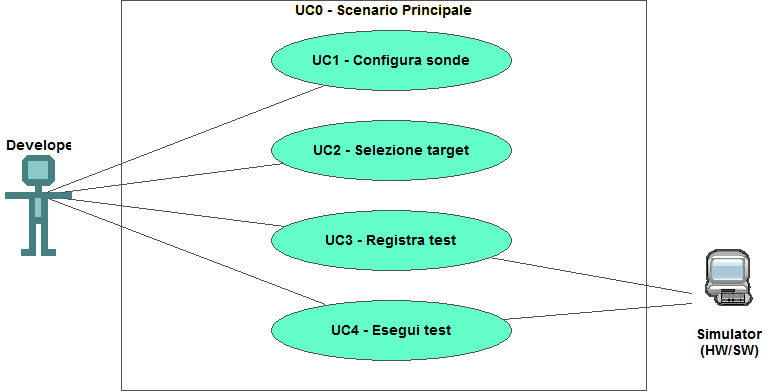
\includegraphics[width=0.9\columnwidth]{usecase/scenario-principale} 
% %     \caption{Use Case - UC0: Scenario principale}
% % \end{figure}

% % \begin{usecase}{0}{Scenario principale}
% % \usecaseactors{Sviluppatore applicativi}
% % \usecasepre{Lo sviluppatore è entrato nel plug-in di simulazione all'interno dell'IDE}
% % \usecasedesc{La finestra di simulazione mette a disposizione i comandi per configurare, registrare o eseguire un test}
% % \usecasepost{Il sistema è pronto per permettere una nuova interazione}
% % \label{uc:scenario-principale}
% % \end{usecase}

% % \section{Tracciamento dei requisiti}

% % Da un'attenta analisi dei requisiti e degli use case effettuata sul progetto è stata stilata la tabella che traccia i requisiti in rapporto agli use case.\\
% % Sono stati individuati diversi tipi di requisiti e si è quindi fatto utilizzo di un codice identificativo per distinguerli.\\
% % Il codice dei requisiti è così strutturato R(F/Q/V)(N/D/O) dove:
% % \begin{enumerate}
% % 	\item[R =] requisito
% %     \item[F =] funzionale
% %     \item[Q =] qualitativo
% %     \item[V =] di vincolo
% %     \item[N =] obbligatorio (necessario)
% %     \item[D =] desiderabile
% %     \item[Z =] opzionale
% % \end{enumerate}
% % Nelle tabelle \ref{tab:requisiti-funzionali}, \ref{tab:requisiti-qualitativi} e \ref{tab:requisiti-vincolo} sono riassunti i requisiti e il loro tracciamento con gli use case delineati in fase di analisi.

% % \newpage

% % \begin{table}%
% % \caption{Tabella del tracciamento dei requisti funzionali}
% % \label{tab:requisiti-funzionali}
% % \begin{tabularx}{\textwidth}{lXl}
% % \hline\hline
% % \textbf{Requisito} & \textbf{Descrizione} & \textbf{Use Case}\\
% % \hline
% % RFN-1     & L'interfaccia permette di configurare il tipo di sonde del test & UC1 \\
% % \hline
% % \end{tabularx}
% % \end{table}%

% % \begin{table}%
% % \caption{Tabella del tracciamento dei requisiti qualitativi}
% % \label{tab:requisiti-qualitativi}
% % \begin{tabularx}{\textwidth}{lXl}
% % \hline\hline
% % \textbf{Requisito} & \textbf{Descrizione} & \textbf{Use Case}\\
% % \hline
% % RQD-1    & Le prestazioni del simulatore hardware deve garantire la giusta esecuzione dei test e non la generazione di falsi negativi & - \\
% % \hline
% % \end{tabularx}
% % \end{table}%

% % \begin{table}%
% % \caption{Tabella del tracciamento dei requisiti di vincolo}
% % \label{tab:requisiti-vincolo}
% % \begin{tabularx}{\textwidth}{lXl}
% % \hline\hline
% % \textbf{Requisito} & \textbf{Descrizione} & \textbf{Use Case}\\
% % \hline
% % RVO-1    & La libreria per l'esecuzione dei test automatici deve essere riutilizzabile & - \\
% % \hline
% % \end{tabularx}
% % \end{table}%
